\documentclass[pdftex,aspectratio=169]{beamer}

% Setup UTF-8 encoding
\usepackage[utf8]{inputenc}
\usepackage[T1]{fontenc}

%\usepackage{flashmovie}

% Setup beamer look theme
\mode<presentation>
{
	\useinnertheme{rectangles}
	\useoutertheme{infolines}
%	\usecolortheme{crane}
%	\usecolortheme{dove}
	\usecolortheme{seagull}
	\setbeamertemplate{navigation symbols}{}
}

% Use nicer font
\usepackage{palatino}
\usepackage{palatino,graphics,array}


% Setup czech language
\usepackage[czech]{babel}

% Include usefull packages
\usepackage{graphics}

% Include hyperlinks support
\usepackage{hyperref}
\hypersetup{colorlinks=true,linkcolor=black,urlcolor=black,unicode=true}

% Add support for simple URLs
\usepackage{url}

\usepackage{tikz}

\usepackage{verbatim}
\usetikzlibrary{arrows,shapes}
\usetikzlibrary{mindmap,trees}


% Commands for CC license
\newcommand{\CcLongnameByNcSa}{\href{http://creativecommons.org/licenses/by-nc-sa/3.0/cz/}{Attribution-Noncommercial-ShareAlike}}
\newcommand{\CcImageBy}[1]{
\includegraphics[scale=#1]{graphics/cc-by-white.pdf}}
\newcommand{\CcImageNc}[1]{
\includegraphics[scale=#1]{graphics/cc-nc-white.pdf}}
\newcommand{\CcImageSa}[1]{
\includegraphics[scale=#1]{graphics/cc-sa-white.pdf}}
\newcommand{\CcGroupByNcSa}[2]{\CcImageBy{#1}\hspace*{#2}\CcImageNc{#1}\hspace*{#2}\CcImageSa{#1}}




\title{User model for the grid}
\subtitle{analysing the impact of different scheduling algorithms}
\author[]{Mgr.~Šimon~Tóth}
\institute[FI@MU]{Faculty of Informatics @ Masaryk University}
\date{\today}

\begin{document}

\begin{frame}
	\titlepage
\end{frame}

\section{Scheduling}

\subsection{Parallel job scheduling problem}

\begin{frame}
	\frametitle{Parallel job scheduling problem}
	\begin{tikzpicture}[auto,
		singlejob/.style = {rectangle, minimum height = 1cm, minimum width = 2cm, fill=blue!20, thick, outer sep=0pt, inner sep=0pt, text centered},
		doublejob/.style = {rectangle, minimum height = 1cm, minimum width = 4.1cm, fill=blue!20, thick, inner sep = 0pt, text centered}
	]
		\matrix[column sep=0.1cm, row sep=0.1cm, ampersand replacement=\& ] {
			\node[rectangle, minimum height = 1cm, minimum width = 1cm ] (user1) { $User_1$ }; \\
			\node[rectangle, minimum height = 1cm, minimum width = 1cm ] (user2) { $User_2$ }; \\
		};
		\node[draw, singlejob, minimum width = 4.5cm, right=0.1cm of user1] (job1) {$Job_1$};
		\node[draw, singlejob, minimum width = 1.8cm, right=0.1cm of job1] {$Job_2$};
		\node[draw, singlejob, minimum width = 2.3cm, right=0.1cm of user2] (job3) {$Job_3$};
		\node[draw, singlejob, minimum width = 1.6cm, right=0.1cm of job3] (job4) {$Job_4$};
		\node[draw, singlejob, minimum width = 1.2cm, right=0.1cm of job4] {$Job_5$};
	\end{tikzpicture}
\end{frame}

\begin{frame}
	\frametitle{Parallel job scheduling problem}
	\begin{tikzpicture}[auto,
		singlejob/.style = {rectangle, minimum height = 1cm, minimum width = 2cm, fill=blue!20, thick, outer sep=0pt, inner sep=0pt, text centered},
		doublejob/.style = {rectangle, minimum height = 1cm, minimum width = 4.1cm, fill=blue!20, thick, inner sep = 0pt, text centered}
	]
		\matrix[column sep=0.1cm, row sep=0.1cm, ampersand replacement=\& ] {
			\node[rectangle, minimum height = 1cm, minimum width = 1cm ] (mach1) { $Resc_1$ }; \\
			\node[rectangle, minimum height = 1cm, minimum width = 1cm ] (mach2) { $Resc_2$ }; \\
			\node[rectangle, minimum height = 1cm, minimum width = 1cm ] (mach3) { $Resc_3$ }; \\
		};
		\node[draw, singlejob, minimum width = 4.5cm, right=0.1cm of mach2] (job1) {$Job_1$};
		\node[draw, singlejob, minimum width = 2.3cm, right=0.1cm of mach1] (job3) {$Job_3$};
		\node[draw, singlejob, minimum width = 1.6cm, right=0.1cm of mach3] (job4) {$Job_4$};
		\node[draw, singlejob, minimum width = 1.2cm, right=0.1cm of job3] (job5) {$Job_5$};
		\node[draw, singlejob, minimum width = 1.8cm, right=0.1cm of job4] (job2){$Job_2$};
	\end{tikzpicture}
	\vfill
\end{frame}

\subsection{Specifics of GRID}

\begin{frame}
	\frametitle{Problem specifics in GRID context}
	\begin{itemize}
		\item multi-dimensional
		\begin{itemize}
			\item each job can request a large set of resources
			\item CPU, Memory, GPU, Scratch, Licenses,...
		\end{itemize}
		\item on-line
		\begin{itemize}
			\item jobs are not known until they arrive into the system
			\item at any time any amount of jobs from any user can arrive
		\end{itemize}
		\item non-clairvoyant
		\begin{itemize}
			\item we only have upper bounds for job run times
			\item jobs appearing as 24 hour long can easily end in 10 minutes
		\end{itemize}
	\end{itemize}
\end{frame}

\subsection{Metrics}

\begin{frame}
	\frametitle{Parallel job scheduling problem}
	\begin{columns}
	\column{0.40\textwidth}
		\begin{tikzpicture}[auto,
			singlejob/.style = {rectangle, minimum height = 1cm, minimum width = 2cm, fill=blue!20, thick, outer sep=0pt, inner sep=0pt, text centered},
			doublejob/.style = {rectangle, minimum height = 1cm, minimum width = 4.1cm, fill=blue!20, thick, inner sep = 0pt, text centered}
		]
			\matrix[column sep=0.1cm, row sep=0.1cm, ampersand replacement=\& ] {
				\node[rectangle, minimum height = 1cm, minimum width = 1cm ] (mach1) { $Resc_1$ }; \\
				\node[rectangle, minimum height = 1cm, minimum width = 1cm ] (mach2) { $Resc_2$ }; \\
				\node[rectangle, minimum height = 1cm, minimum width = 1cm ] (mach3) { $Resc_3$ }; \\
			};
			\node[draw, singlejob, minimum width = 4.5cm, right=0.1cm of mach2] (job1) {$Job_1$};
			\node[draw, singlejob, minimum width = 2.3cm, right=0.1cm of mach1] (job3) {$Job_3$};
			\node[draw, singlejob, minimum width = 1.6cm, right=0.1cm of mach3] (job4) {$Job_4$};
			\node[draw, singlejob, minimum width = 1.2cm, right=0.1cm of job3] (job5) {$Job_5$};
			\node[draw, singlejob, minimum width = 1.8cm, right=0.1cm of job4] (job2){$Job_2$};
		\end{tikzpicture}
		\vfill
	\column{0.55\textwidth}
		\visible<2->{
		\begin{tikzpicture}[auto,
			singlejob/.style = {rectangle, minimum height = 1cm, minimum width = 2cm, fill=blue!20, thick, outer sep=0pt, inner sep=0pt, text centered},
			doublejob/.style = {rectangle, minimum height = 1cm, minimum width = 4.1cm, fill=blue!20, thick, inner sep = 0pt, text centered}
		]
			\matrix[column sep=0.1cm, row sep=0.1cm, ampersand replacement=\& ] {
				\node[rectangle, minimum height = 1cm, minimum width = 1cm ] (mach1) { $Resc_1$ }; \\
				\node[rectangle, minimum height = 1cm, minimum width = 1cm ] (mach2) { $Resc_2$ }; \\
				\node[rectangle, minimum height = 1cm, minimum width = 1cm ] (mach3) { $Resc_3$ }; \\
			};
			\node[draw, singlejob, minimum width = 2.3cm, right=0.1cm of mach2] (job3) {$Job_3$};
			\node[draw, singlejob, minimum width = 1.6cm, right=0.1cm of mach3] (job4) {$Job_4$};
			\node[draw, singlejob, minimum width = 1.2cm, right=0.1cm of mach1] (job5) {$Job_5$};
			\node[draw, singlejob, minimum width = 1.8cm, right=0.1cm of job3] (job2){$Job_2$};
			\node[draw, singlejob, minimum width = 4.5cm, right=0.1cm of job5] (job1) {$Job_1$};
		\end{tikzpicture}
		}
		\vfill
	\end{columns}
\end{frame}

\begin{frame}
	\frametitle{Metrics}
	\begin{columns}
	\column{0.45\textwidth}
		\begin{itemize}
			\item performance metrics
				\begin{itemize}
					\item system oriented
					\item user/job oriented
				\end{itemize}
			\item fairness metrics
		\end{itemize}
	\column{0.45\textwidth}
	\visible<2->{
		\begin{tikzpicture}[thick]
			\filldraw[fill=blue!20] (3,0) rectangle (6,1);
			\draw (3,0.5) -- (1,0.5);
			\draw (1,0.34) -- (1,0.66);
			\node at (1,1.5) (arr) {arrival};
			\node at (3,1.5) (sta) {start};
			\node at (6,1.5) (end) {end};
			\draw [thick, decoration={ brace, mirror, raise=0.5cm },  decorate ] (1,0) -- (2.9,0) node [pos=0.5,anchor=north,yshift=-0.55cm] {waittime};
			\draw [thick, decoration={ brace, mirror, raise=0.5cm },  decorate ] (3.1,0) -- (6,0) node [pos=0.5,anchor=north,yshift=-0.55cm] {run-time};
			\draw [thick, decoration={ brace, mirror, raise=0.5cm },  decorate ] (1,-1) -- (6,-1) node [pos=0.5,anchor=north,yshift=-0.55cm] {response};
		\end{tikzpicture}
		}
	\end{columns}
\end{frame}

\begin{frame}
	\frametitle{Example of bad evaluation}
	\begin{tikzpicture}[auto,
		singlejob/.style = {rectangle, minimum height = 1cm, minimum width = 2cm, fill=blue!20, thick, outer sep=0pt, inner sep=0pt, text centered},
		doublejob/.style = {rectangle, minimum height = 1cm, minimum width = 4.1cm, fill=blue!20, thick, inner sep = 0pt, text centered}
	]
		\matrix[column sep=0.1cm, row sep=0.1cm, ampersand replacement=\& ] {
			\node[rectangle, minimum height = 1cm, minimum width = 1cm ] { $Resc_1$ };\&
			\node[draw, singlejob] {$Job_1$};\& \node[draw, singlejob] {$Job_2$};\&
			\node[draw, singlejob] {$Job_3$};\& \node[draw, singlejob] {$Job_4$}; \\

			\node[rectangle, minimum height = 1cm, minimum width = 1cm ] { $Resc_2$ };\&
			\node[singlejob] (j51) {}; \& \node[singlejob] (j52) {}; \&
			\node[singlejob] (j61) {}; \& \node[singlejob] (j62) {}; \\
		};
		\node[draw,doublejob,fill=red!20] (outer) [fit=(j51) (j52),label=center:$Job_5$] {};
		\node[draw,doublejob,fill=red!20] (outer) [fit=(j61) (j62),label=center:$Job_6$] {};
	\end{tikzpicture}
\end{frame}

\begin{frame}
	\frametitle{Example of bad evaluation}
	\begin{tikzpicture}[auto,
		singlejob/.style = {rectangle, minimum height = 1cm, minimum width = 2cm, fill=blue!20, thick, outer sep=0pt, inner sep=0pt, text centered},
		doublejob/.style = {rectangle, minimum height = 1cm, minimum width = 2cm, fill=blue!20, thick, inner sep = 0pt, text centered}
	]
		\matrix[column sep=0.1cm, row sep=0.1cm, ampersand replacement=\& ] {
			\node[rectangle, minimum height = 1cm, minimum width = 1cm ] { $Resc_1$ };\&
			\node[draw, singlejob] {$Job_1$};\& \node[draw, singlejob] {$Job_3$};\& \node[draw, singlejob] {$Job_5$};\& \node[draw, singlejob] {$Job_7$}; \\

			\node[rectangle, minimum height = 1cm, minimum width = 1cm ] { $Resc_2$ };\&
			\node[draw, singlejob] {$Job_2$};\& \node[draw, singlejob] {$Job_4$};\& \node[draw, singlejob] {$Job_6$};\& \node[draw, singlejob] {$Job_8$}; \\

			\node[rectangle, minimum height = 1cm, minimum width = 1cm ] { $Resc_3$ };\&
			\node[singlejob] (j51) {}; \& \node[singlejob] (j61) {}; \& \node[singlejob] (j71) {}; \& \node[singlejob] (j81) {}; \\
			\node[rectangle, minimum height = 1cm, minimum width = 1cm ] { $Resc_4$ };\&
			\node[singlejob] (j52) {}; \& \node[singlejob] (j62) {}; \& \node[singlejob] (j72) {}; \& \node[singlejob] (j82) {}; \\
		};
		\node[draw,doublejob,fill=red!20] (outer) [fit=(j51) (j52),label=center:$Job_{10}$] {};
		\node[draw,doublejob,fill=red!20] (outer) [fit=(j61) (j62),label=center:$Job_{11}$] {};
		\node[draw,doublejob,fill=red!20] (outer) [fit=(j71) (j72),label=center:$Job_{12}$] {};
		\node[draw,doublejob,fill=red!20] (outer) [fit=(j81) (j82),label=center:$Job_{13}$] {};
	\end{tikzpicture}
\end{frame}

\begin{frame}
	\frametitle{Metrics}
	\begin{columns}
	\column{0.45\textwidth}
		\begin{itemize}
			\item performance metrics
				\begin{itemize}
					\item system oriented
					\item user/job oriented
				\end{itemize}
			\item fairness metrics
		\end{itemize}
	\column{0.45\textwidth}
		
	\end{columns}
\end{frame}

\subsection{Concept of fairness}

\begin{frame}
	\frametitle{Fairness}
	\begin{itemize}
		\item many different representations
		\item MetaCentrum uses algorithmic approach
		\begin{itemize}
			\item priority balancing algorithm
			\item using the system decreases priority
		\end{itemize}
	\end{itemize}

	\begin{align*}
	& \forall i; \lim_{time \to \infty} Usage(User_i) = TotalUsage \times DesignatedFraction(User_i)
	\end{align*}
\end{frame}

\subsection{Applying metrics}

\begin{frame}
	\frametitle{Applying metrics}
	\begin{columns}
	\column{0.45\textwidth}
		\begin{itemize}
			\item metrics are not independent
			\item requirements are very vague
		\end{itemize}
	\column{0.45\textwidth}
		\begin{tikzpicture}
		\path[coordinate] (0,0)  coordinate(A)
	                ++( 60:5cm) coordinate(B)
	                ++(-60:5cm) coordinate(C);
		\draw[fill=blue!20] (A) -- (B) -- (C) -- cycle;
		\node at (0,-0.5cm) (bl) {job metrics};
		\node at (5cm,-0.5cm) (br) {system metrics};
		\node at (2.5cm,4.7cm) (top) {fairness};
		\end{tikzpicture}
	\end{columns}
\end{frame}

\section{Quantifying the quality}
\subsection{The model}

\begin{frame}
	\frametitle{Back to fundamentals}
	\begin{itemize}
		\item quality based of user satisfaction
		\item modelling user expectations
	\end{itemize}
\end{frame}

\begin{frame}
	\frametitle{The model}
	\begin{itemize}
		\item each user given "bandwidth"
		\begin{itemize}
			\item CPU $8\frac{core}{second}$
			\item memory $16\frac{GB}{second}$
		\end{itemize}
		\item for each job a deadline is calculated according to available bandwidth
	\end{itemize}
\end{frame}

\begin{frame}
	\frametitle{Deadlines example}
	4 jobs
	\begin{itemize}
		\item 4 CPU cores
		\item 8 GB RAM
		\item 4 hour runtime
	\end{itemize}
	Deadlines:
	\begin{itemize}
		\item 4 hours for first and second job
		\item 8 hours for third and fourth job
	\end{itemize}
\end{frame}

\section{Examples of results}
\subsection{Comparing different simple algorithms}

\begin{frame}
	\frametitle{Alea - the Grid Simulation Environment}
	\begin{itemize}
		\item created by RNDr. Dalibor Klusáček, Ph.D.
		\item uses real data sets from CERIT and MetaCentrum
	\end{itemize}
\end{frame}

\begin{frame}
	\frametitle{Scheduling algorithms}
	\begin{itemize}
		\item trivial FIFO
		\item FIFO with backfilling
		\item combinations with fairshare variants
	\end{itemize}
\end{frame}

\begin{frame}
	\frametitle{Overview graphs}
	\begin{center}
	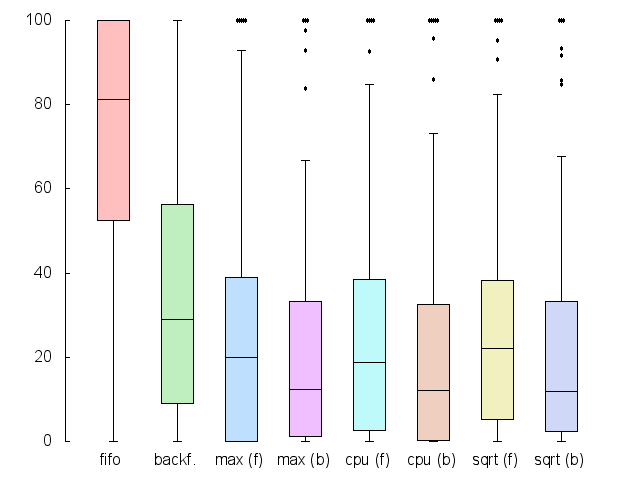
\includegraphics[width=0.6\textwidth]{perc_deadline.png}
	\end{center}
\end{frame}

{
\usebackgroundtemplate{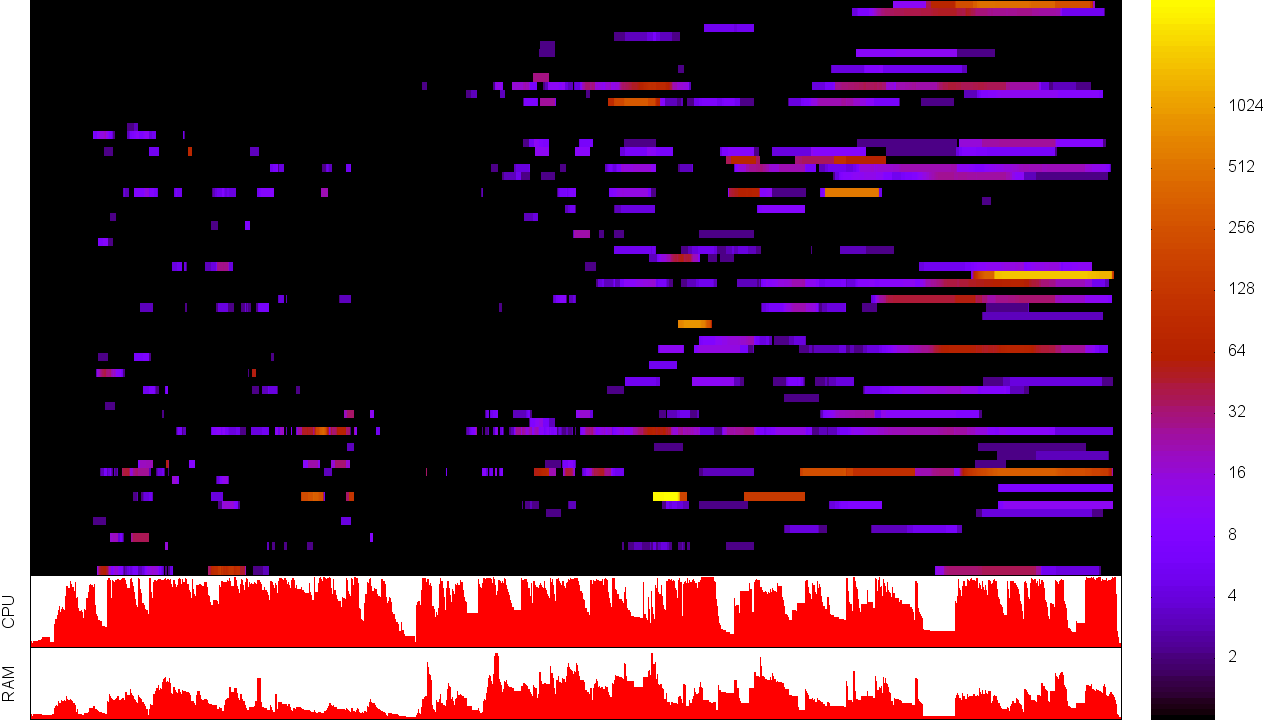
\includegraphics[width=\paperwidth]{outputs/none_fifo.png}}
\begin{frame}[plain]
\begin{minipage}[t][\textheight]{\textwidth}
	\color{white}\textbf{Trivial FIFO}
\end{minipage}
\end{frame}
}

{
\usebackgroundtemplate{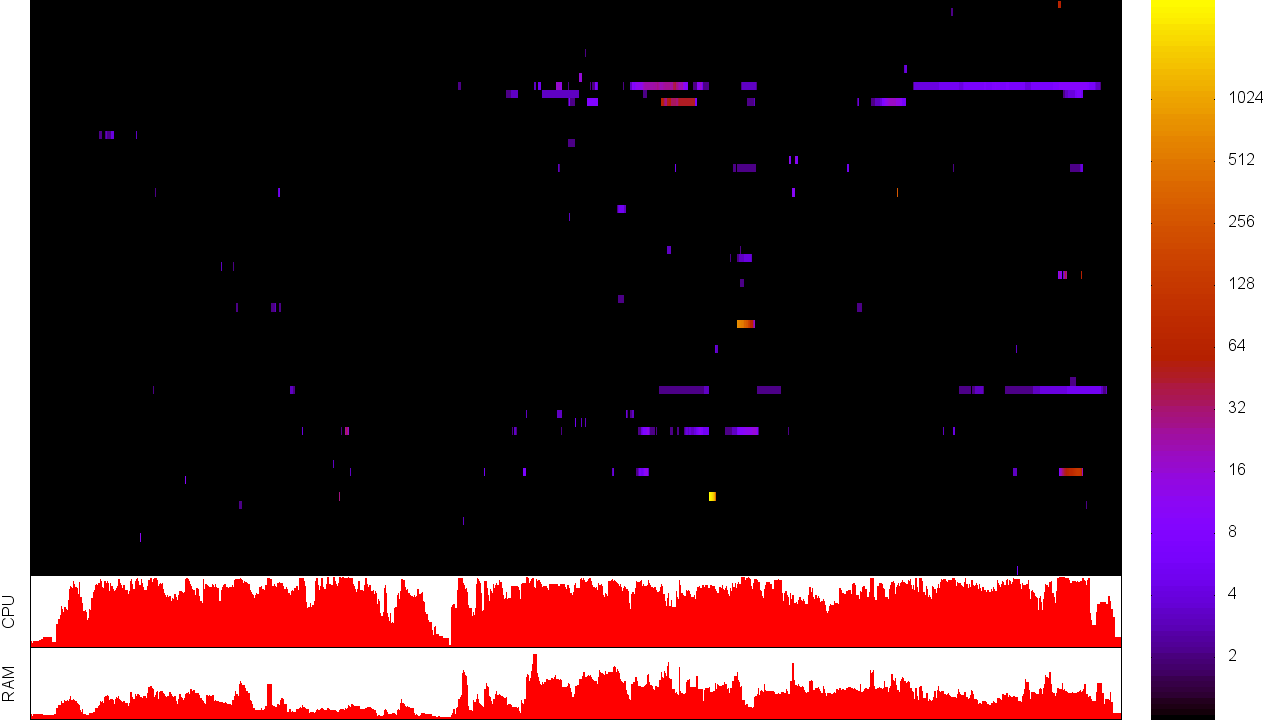
\includegraphics[width=\paperwidth]{outputs/max_backfill.png}}
\begin{frame}[plain]
\begin{minipage}[t][\textheight]{\textwidth}
	\color{white}\textbf{Backfilling}
\end{minipage}
\end{frame}
}

{
\usebackgroundtemplate{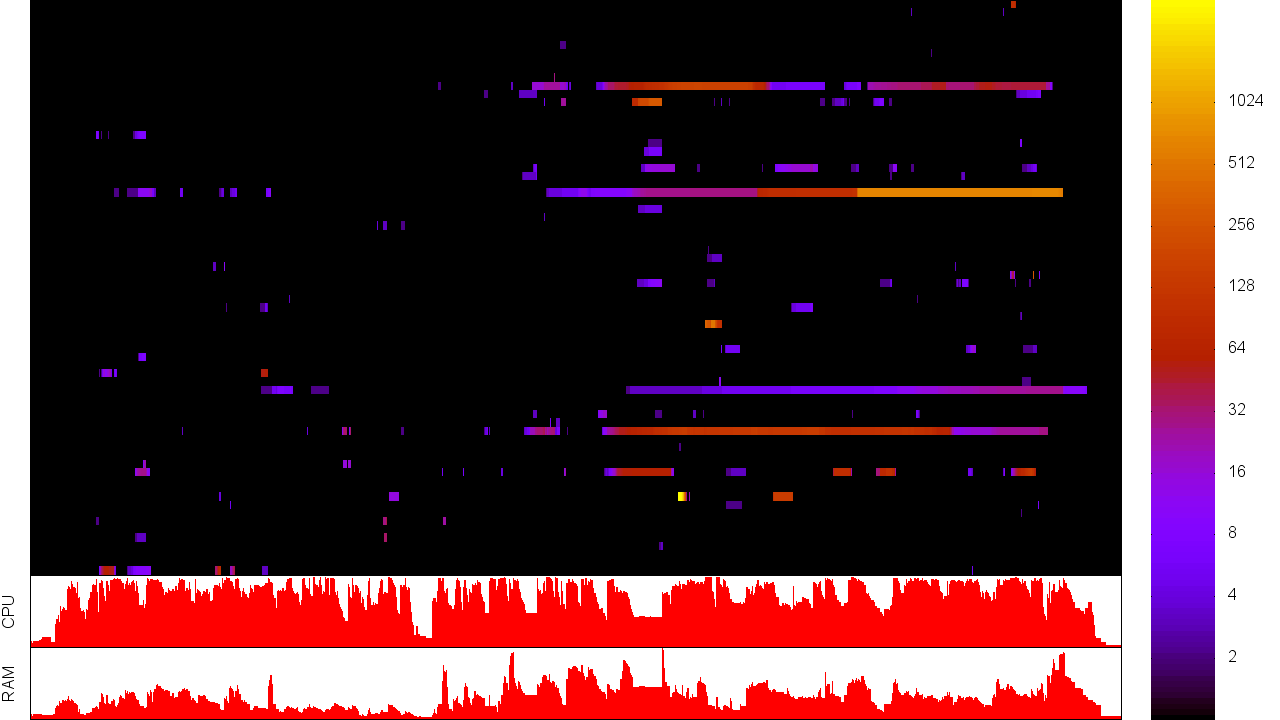
\includegraphics[width=\paperwidth]{outputs/max_fifo.png}}
\begin{frame}[plain]
\begin{minipage}[t][\textheight]{\textwidth}
	\color{white}\textbf{Fairshare}
\end{minipage}
\end{frame}
}

{
\usebackgroundtemplate{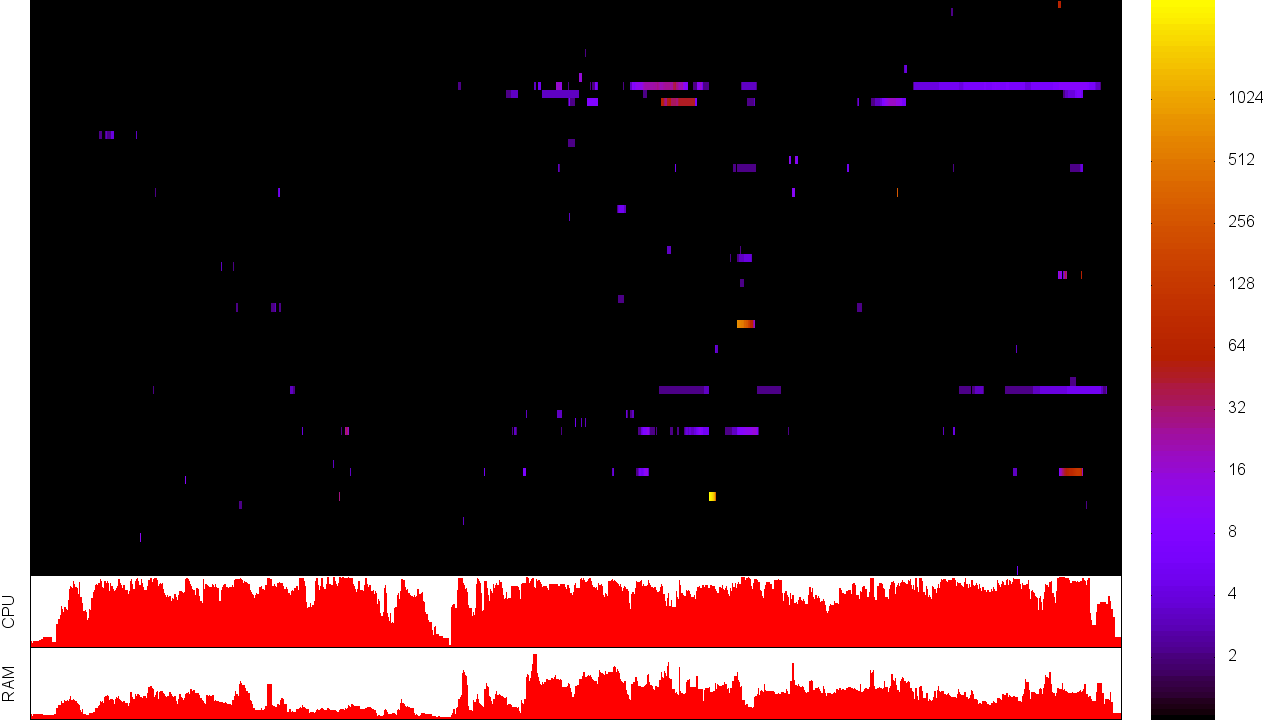
\includegraphics[width=\paperwidth]{outputs/max_backfill.png}}
\begin{frame}[plain]
\begin{minipage}[t][\textheight]{\textwidth}
	\color{white}\textbf{Fairshare \& Backfilling}
\end{minipage}
\end{frame}
}

{
\usebackgroundtemplate{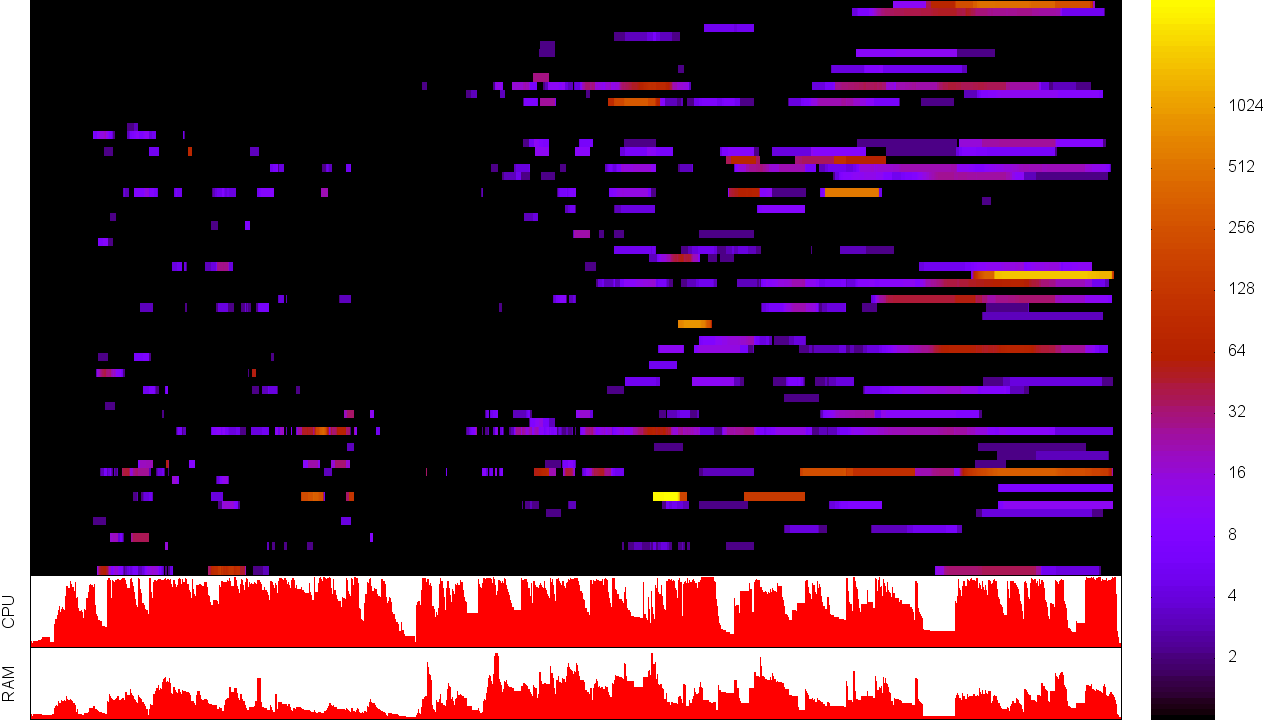
\includegraphics[width=\paperwidth]{outputs/none_fifo.png}}
\begin{frame}[plain]
\begin{minipage}[t][\textheight]{\textwidth}
	\color{white}\textbf{Trivial FIFO}
\end{minipage}
\end{frame}
}

{
\usebackgroundtemplate{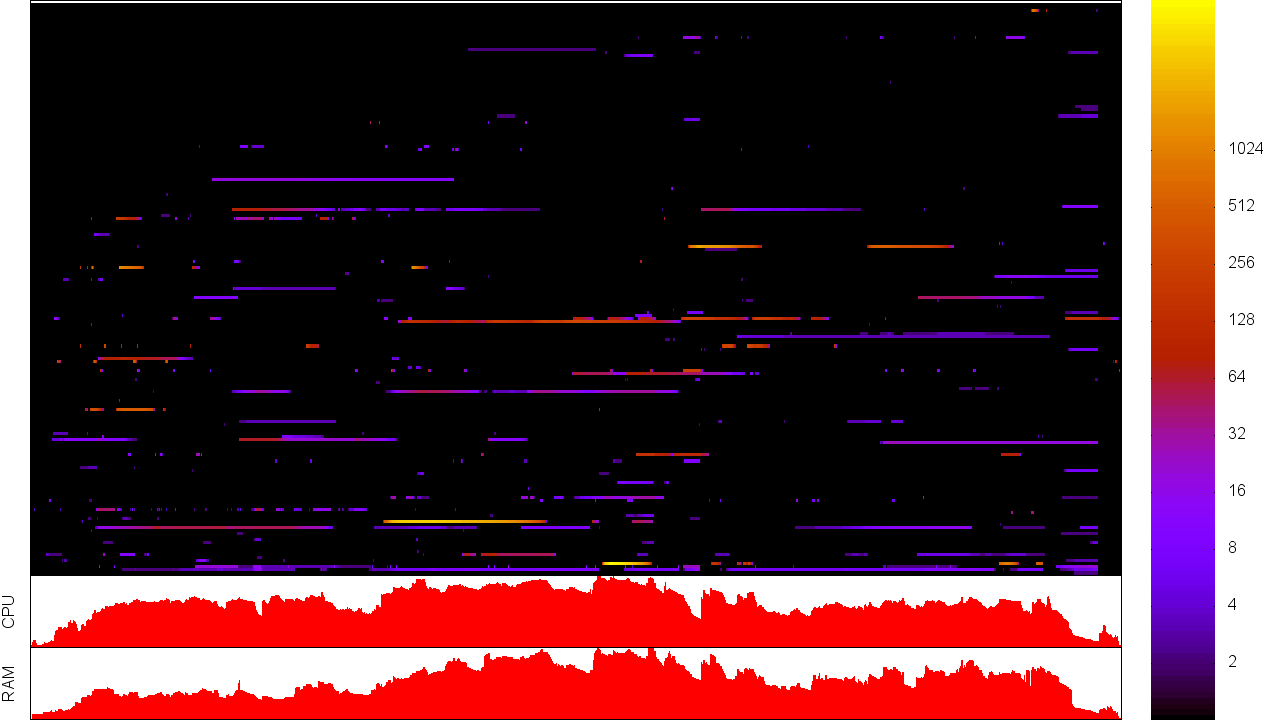
\includegraphics[width=\paperwidth]{outputs/metacentrum1.png}}
\begin{frame}[plain]
\begin{minipage}[t][\textheight]{\textwidth}
	\color{white}\textbf{MetaCentrum}
\end{minipage}
\end{frame}
}

{
\usebackgroundtemplate{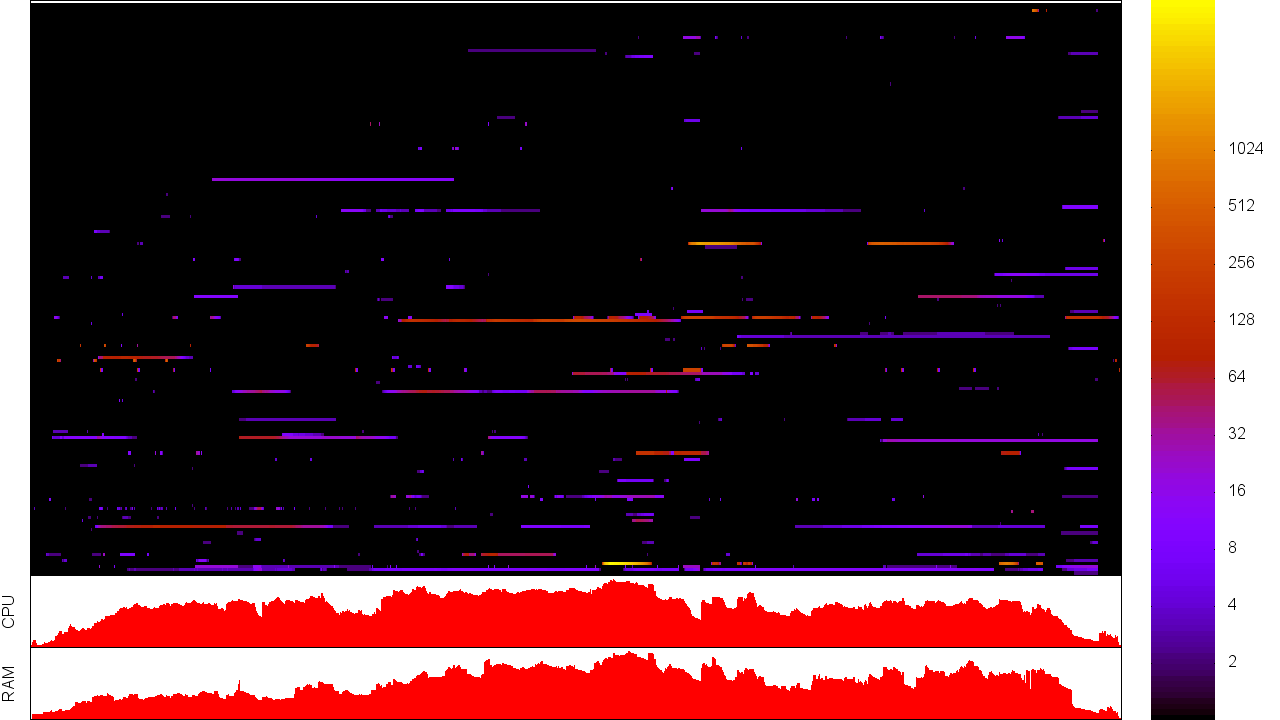
\includegraphics[width=\paperwidth]{outputs/metacentrum2.png}}
\begin{frame}[plain]
\begin{minipage}[t][\textheight]{\textwidth}
	\color{white}\textbf{MetaCentrum - backfill queue}
\end{minipage}
\end{frame}
}

{
\usebackgroundtemplate{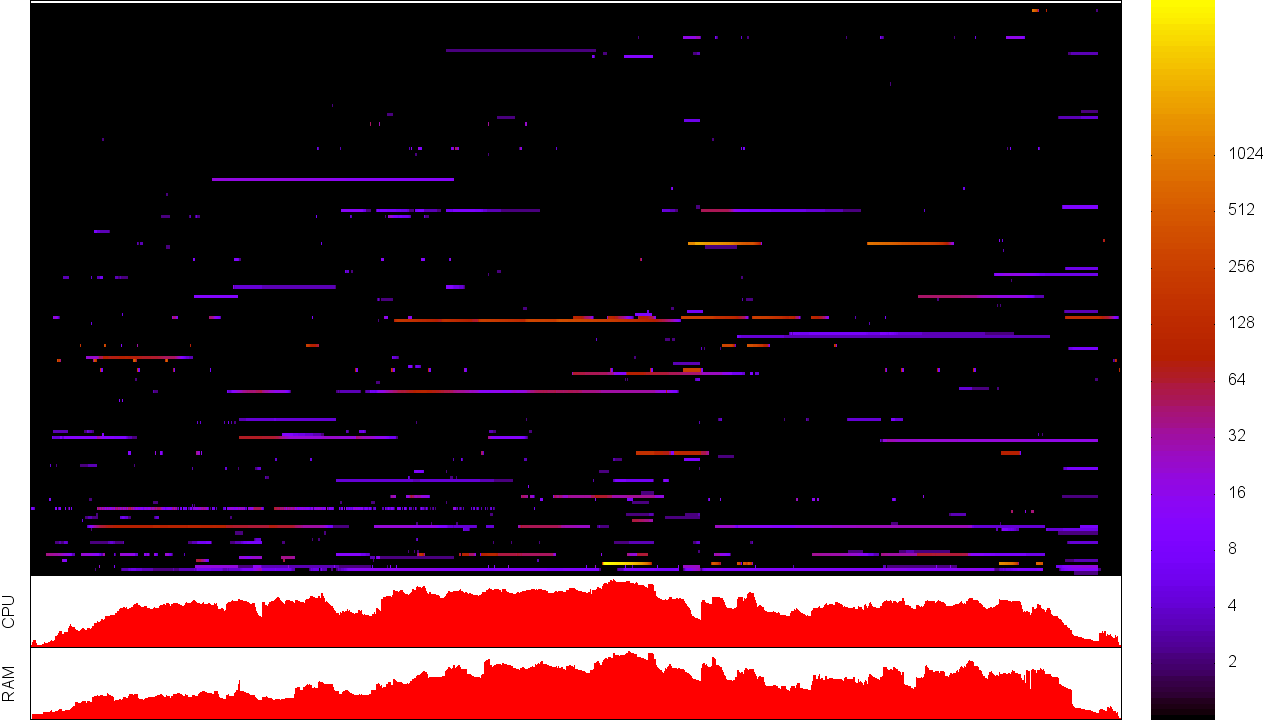
\includegraphics[width=\paperwidth]{outputs/metacentrum3.png}}
\begin{frame}[plain]
\begin{minipage}[t][\textheight]{\textwidth}
	\color{white}\textbf{Metacentrum}
\end{minipage}
\end{frame}
}







\subsection{Future work}

\begin{frame}
	\frametitle{Future work}
	\begin{itemize}
		\item users with different priorities \pause
		\item users with different tolerance towards deadline violation \pause
		\item users with special access to particular machines
	\end{itemize}
\end{frame}

\section{Conclusion}
\subsection{Summary}

\begin{frame}
	\frametitle{Summary}
	\begin{itemize}
		\item new independent model for analysing generated schedules
		\item modeling user expectations
		\item deadline based model
		\item highly configurable
	\end{itemize}
\end{frame}

\subsection{The End}

\begin{frame}
	\hspace{0.7cm}
		
\includegraphics[width=0.2\textwidth]{filogo.pdf}
	\hspace{1cm}
	\begin{minipage}[b]{0.3\textwidth}
		
\includegraphics[width=\textwidth]{cesnet-logo-800.png}\newline
		
\includegraphics[width=\textwidth]{metalogo1.png}
	\end{minipage}
	\hspace{0.4cm}
	\begin{minipage}[b]{0.3\textwidth}
	
\includegraphics[width=\textwidth]{cerit-sc-logo.png}
	\vspace{1cm}
\end{minipage}
\end{frame}


\end{document}
